\documentclass[11pt,a4paper,landscape]{article}
\usepackage[margin=12mm]{geometry}
\usepackage{fontspec,xeCJK}
\setmainfont{Arial}
\setCJKmainfont{Yu Gothic}
\usepackage{graphicx,booktabs,xcolor,amsmath,xurl}
\urlstyle{tt}
\definecolor{ink}{HTML}{263D50}
\setlength{\parindent}{0pt}
\setlength{\parskip}{4pt}
\newcommand{\heading}[2]{{\LARGE\bfseries\color{ink}#1}\par{\small #2}\par\vspace{1mm}}
\begin{document}
\heading{GAの最大カット値を、多様性の色で追跡する}
{G22・G55・G70、全ランダム／全CIM初期集団、各16 run・300世代。保存済み軌跡の再描画}

\begin{center}
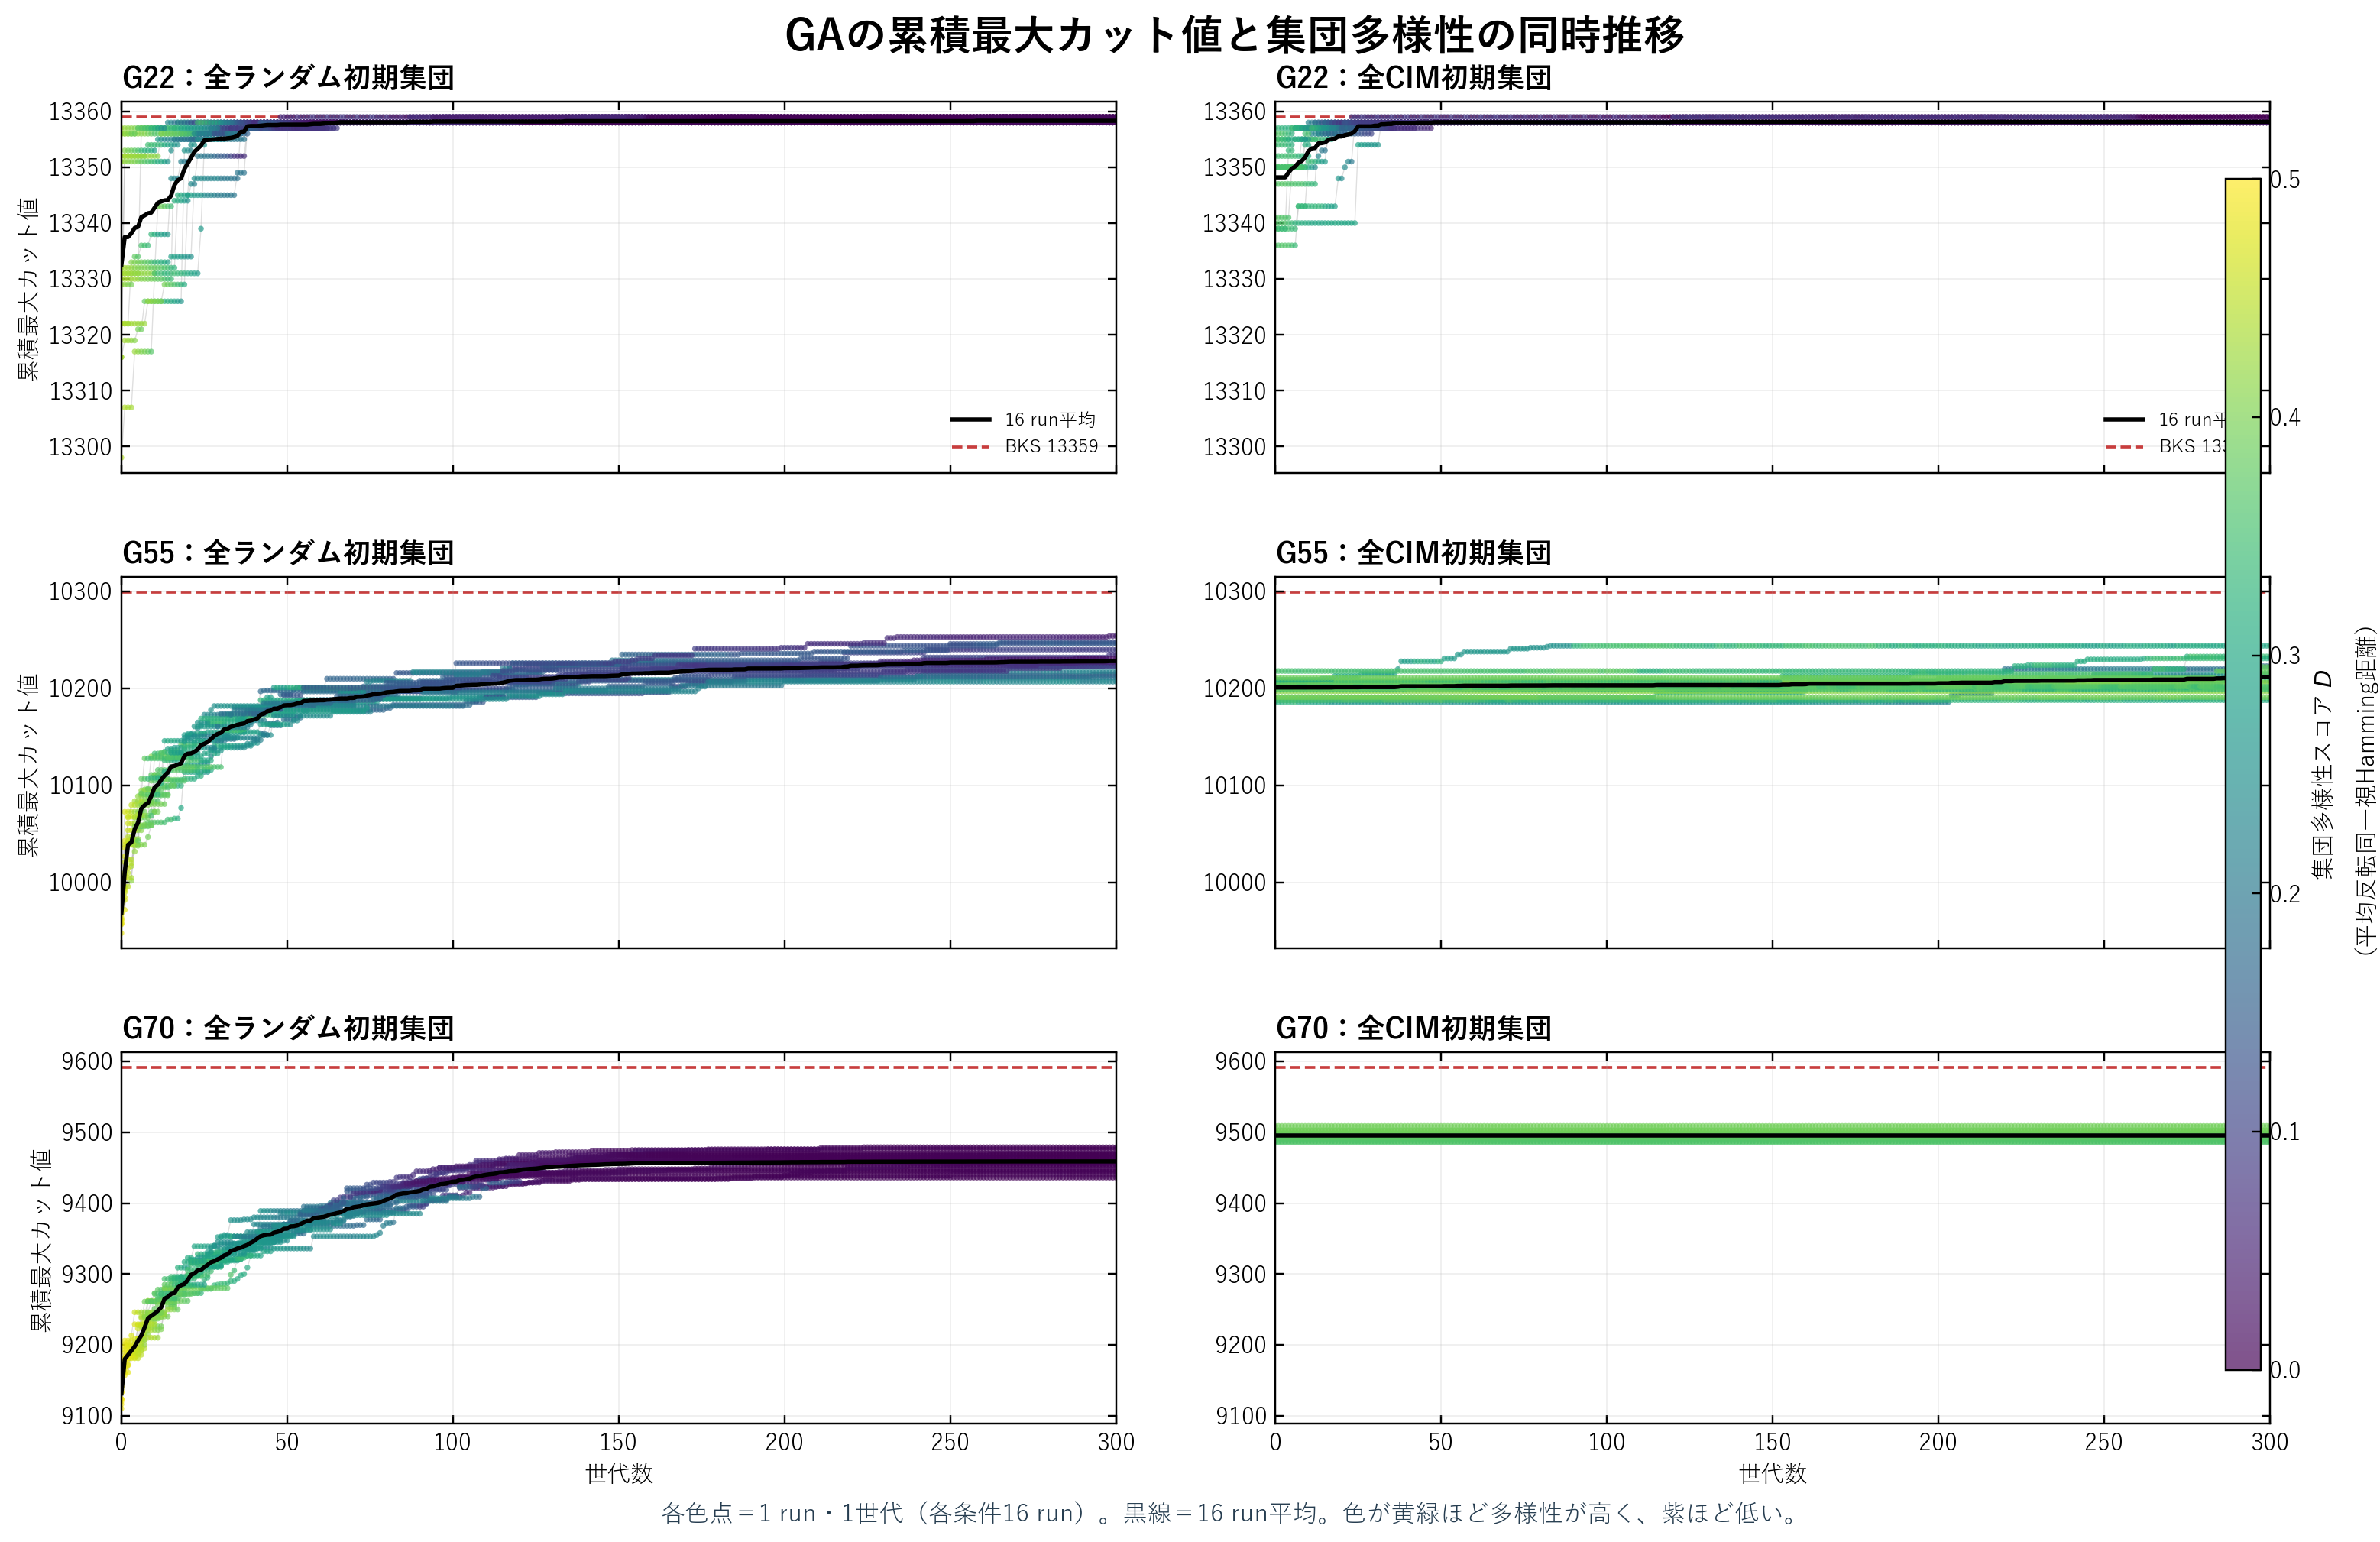
\includegraphics[width=0.97\linewidth,height=159mm,keepaspectratio]{trajectory.png}
\end{center}

{\small \textbf{点の定義：}各点は「1 run・1世代」。横軸は世代数、縦軸はそのrunがその世代までに見つけた累積最大カット値、色は同じrun・同じ世代の集団多様性$D$。黒線は16 run平均、赤破線はBKS。$D=\operatorname{mean}_{i<j}\min(H_{ij},N-H_{ij})/N$で、全反転は同じ分割として扱う。}

\clearpage
\heading{開始時と300世代後の数値}{世代0は初期集団の全個体にTabu Searchを適用した後}

\begin{center}\small
\begin{tabular}{llrrrrr}\toprule
問題 & 初期集団 & 世代0最良値 & 世代300最良値 & 改善量 & 世代0の$D$ & 世代300の$D$ \\\midrule
G22 & 全ランダム初期集団 & 13332.56 & 13358.31 & 25.75 & 0.4345 & 0.0138 \\
G22 & 全CIM初期集団 & 13348.19 & 13358.12 & 9.94 & 0.3632 & 0.0207 \\
G55 & 全ランダム初期集団 & 9968.75 & 10228.25 & 259.50 & 0.4813 & 0.1024 \\
G55 & 全CIM初期集団 & 10201.06 & 10212.00 & 10.94 & 0.3645 & 0.3380 \\
G70 & 全ランダム初期集団 & 9131.50 & 9458.94 & 327.44 & 0.4895 & 0.0026 \\
G70 & 全CIM初期集団 & 9495.19 & 9495.19 & 0.00 & 0.3755 & 0.3755 \\
\bottomrule\end{tabular}
\end{center}

\textbf{図から読み取れる例}

\begin{itemize}
\item G22では両初期集団とも世代とともに最大カット値が上がり、多様性は低下する。
\item G55の全CIMは比較的高い多様性を保つ点が多いが、最大カット値の改善は小さい。
\item G70の全CIMは多様性がほぼ一定のまま、16 runすべてで最大カット値が改善しない。
\end{itemize}

\colorbox{yellow!18}{\parbox{0.96\linewidth}{\textbf{解釈上の注意：}全ランダムと全CIMでは世代0の品質をそろえていない。この図は最大カット値と多様性の時間的な同時推移を示すが、多様性が改善を引き起こしたという因果関係は示さない。}}

\textbf{再現性}

元データ：\path{results/2026-09-14/ga_diversity_trajectory/v1_G22_G55_G70_nt16_gen300_measured}。解析コード、群集計、入力SHA-256を本PDFと同じフォルダに保存した。元実験では864集団の距離と8352個体のカット値が独立照合済み。
\end{document}
